%%%%%%%%%%%%%%%%%%%%%%
% USYD Biodomain 2016-08-04
% (c) jpb, jan.buchmann@sydney.edu.au
%%%%%%%%%%%%%%%%%%%%%%

\documentclass{beamer}
\usetheme{default}
\beamertemplatenavigationsymbolsempty
\usepackage{xspace}
\usepackage{booktabs}
\usepackage{listings}
\usepackage{multirow}
\usepackage{ifthen}
\usepackage{jpb.pgf}
\lstset{basicstyle=\tiny\ttfamily,breaklines=true}
  \usetikzlibrary{shapes.geometric, positioning, calc, shadings}
  \tikzset{%
  db/.style = {cylinder, draw, fill=white, inner sep=2pt},
  tool/.style = {rectangle, draw, fill=white, inner sep=2pt},
  data/.style = {},
  func/.style = {},
  fake/.style = {},
  dna/.style = {draw, very thick},
  partLabel/.style = {font=\bfseries,
                      fill=gray!10,rounded corners, draw=black!50, dashed},
  every legend to name picture/.style={west}
  }
  \pgfdeclareplotmark{db}{\node [cylinder, draw=black] {};}
  \definecolor{struc}{rgb}{0.8,0.09,0.01}
  \definecolor{func}{rgb}{0.17,0.48,0.71}
  \definecolor{rightfl}{rgb}{0.14,0.75,0.4}
  \definecolor{leftfl}{rgb}{0.64,0.06,0.06}
\usepackage{inconsolata}
\hypersetup{pdfstartview={Fit}}


%%% Titleslide  %%%
\title[]{Endovir}
\subtitle{Report NCBI Visiting Bioinf}
\author[]{Jan P. Buchmann}
\institute{NCBI, NLM, NIH, Bethesda, MD, USA \\
           The University of Sydney, Sydney, Australia}
\date{2017-12-08}
%**************************


\begin{document}
  \titlepage

  \begin{frame}{Exogenous / Endogenous viruses}
    \begin{block}{Exogenous virus}
      \begin{itemize}
       \item Integration into host genome not required for replication
       \item Can occur occasionally, e.g. Human Hepres virus 6
       \item Clearly separated form host genome
      \end{itemize}
      \begin{tikzpicture}[node distance=1cm]
   \tikzset{%
      n/.style = {orf, minimum width=0.7cm},
      m/.style = {orf, minimum width=0.85cm},
      g/.style = {orf, minimum width=0.83cm},
      l/.style = {orf, minimum width=3.2cm},
      }
    \def\d {0.2}

    \node (lead)  [end]                           {3$^{\prime}$};
    \node (n)     [orf, n, right = \d cm of lead] {N};
    \node (m)     [orf, m, right = \d cm of n] {M};
    \node (g)     [orf, g, right = \d cm of m]    {G};
    \node (l)     [orf, l, right = \d cm of g]    {L};
    \node (trail) [end, right = \d cm of l]       {5$^{\prime}$};
    \coordinate (tpos) at ($(lead)!.5!(trail)$);

    \draw[vrsgenome] (lead) -- (n) -- (m) -- (g) -- (l) -- (trail);
    \node at (tpos) [title, above = 1em] {Rabies virus};
    \draw[|-|, semithick] ($(lead.east) + (0, -0.5)$) -- ($(trail.west) + (0, -0.5)$) node[midway, below] {11~kb};

    %\begin{scope}[yshift=-4em]
      %\node (leg0) at (0,0) [draw, orf, fill=struc] {};
      %\node [right = of leg0] {Strucutral ORF};
      %\node (leg1)[below = of leg0] {Strucutral ORF};
    %\end{scope}
\end{tikzpicture}

    \end{block}

    \begin{block}{Endogenous virus}
      \begin{itemize}
       \item Integration into host genome mandatory for replication
       \item Retroviridae, e.g. HIV
       \item Part of the host genome
      \end{itemize}
      \begin{tikzpicture}
  \def\d {0.2}
  \node (lead)    [end]                           {5$^{\prime}$};
  \node (vrsbeg)  [right = 2 cm of lead]          {};
  \node (orf0)    [orf, right = \d cm of vrsbeg]  {ORF1};
  \node (orf1)    [orf, right = \d cm of orf0]    {ORF2};
  \node (orf2)    [orf, right = \d cm of orf1]    {ORF3};
  \node (vrsend)  [right = \d cm of orf2]         {};
  \node (trail)   [end, right = 2 cm of vrsend]     {3$^{\prime}$};
  \draw[hostgenome] (lead) -- (vrsbeg.east);
  \draw[vrsgenome] (vrsbeg) -- (orf0) -- (orf1) -- (orf2) -- (vrsend);
  \draw[hostgenome] (vrsend.west) -- (trail);
  \draw[|-|, semithick] ($(vrsbeg.east) + (0, -0.5)$) -- ($(vrsend.west) + (0, -0.5)$) node [midway, below] {$\le$20~kb};

\end{tikzpicture}

    \end{block}
  \end{frame}

  \begin{frame}{SRA data}
    \begin{itemize}
      \item SRA data contains host and virus sequences
      \item Endogenous and putative novel viruses
    \end{itemize}
    \begin{tikzpicture}
  \def\n {40}
  \def\Ynormfac{7}
  \def\nodeYcoord{\n/2/\Ynormfac}
  \node (vir) [vrsgenomecolor,  font=\small] at (-1,\nodeYcoord) {Virus reads};
  \node (host)[hostgenomecolor, font=\small] at (8,\nodeYcoord) {Host/Sample reads};
  \def\labelYcoord{0}
  \foreach \x in {0,...,\n} % draw n read
  {
    \pgfmathsetmacro{\Ya}{((random(\n)))/\Ynormfac}
    \pgfmathsetmacro{\Xa}{((random(\n)))/8}
    \pgfmathsetmacro{\La}{random()+0.5}
    \def\xcoord{\pgfmathparse{(\La+\Xa)/2)}}
    \ifthenelse{\x>30}
    {
      \draw[vrsgenome, very thick] (\Xa, \Ya) -- (\La+\Xa, \Ya);{}
      \coordinate (x) at (\Xa, \Ya);
      \draw[-, vrsgenomecolor!60,thick, shorten >=0pt,shorten <=2pt] (x) -- (vir.east);
    }
    {
     \draw[hostgenome] (\Xa, \Ya) -- (\La+\Xa, \Ya);{}
     \coordinate (x) at (\Xa+\La, \Ya);
      \draw[-, hostgenomecolor!60, shorten >=0pt,shorten <=1pt] (x) -- (host.west);
    }
  }


\end{tikzpicture}

  \end{frame}

  \begin{frame}{Previous work}
    \begin{itemize}
      \item ViruSpy \footnote{https://github.com/NCBI-Hackathons/ViruSpy}
      \item Logic  mostly implemented in Bash and Perl \\
              $\rightarrow$ Complex to expand and adjust
      \item BUD algorithm
    \end{itemize}
    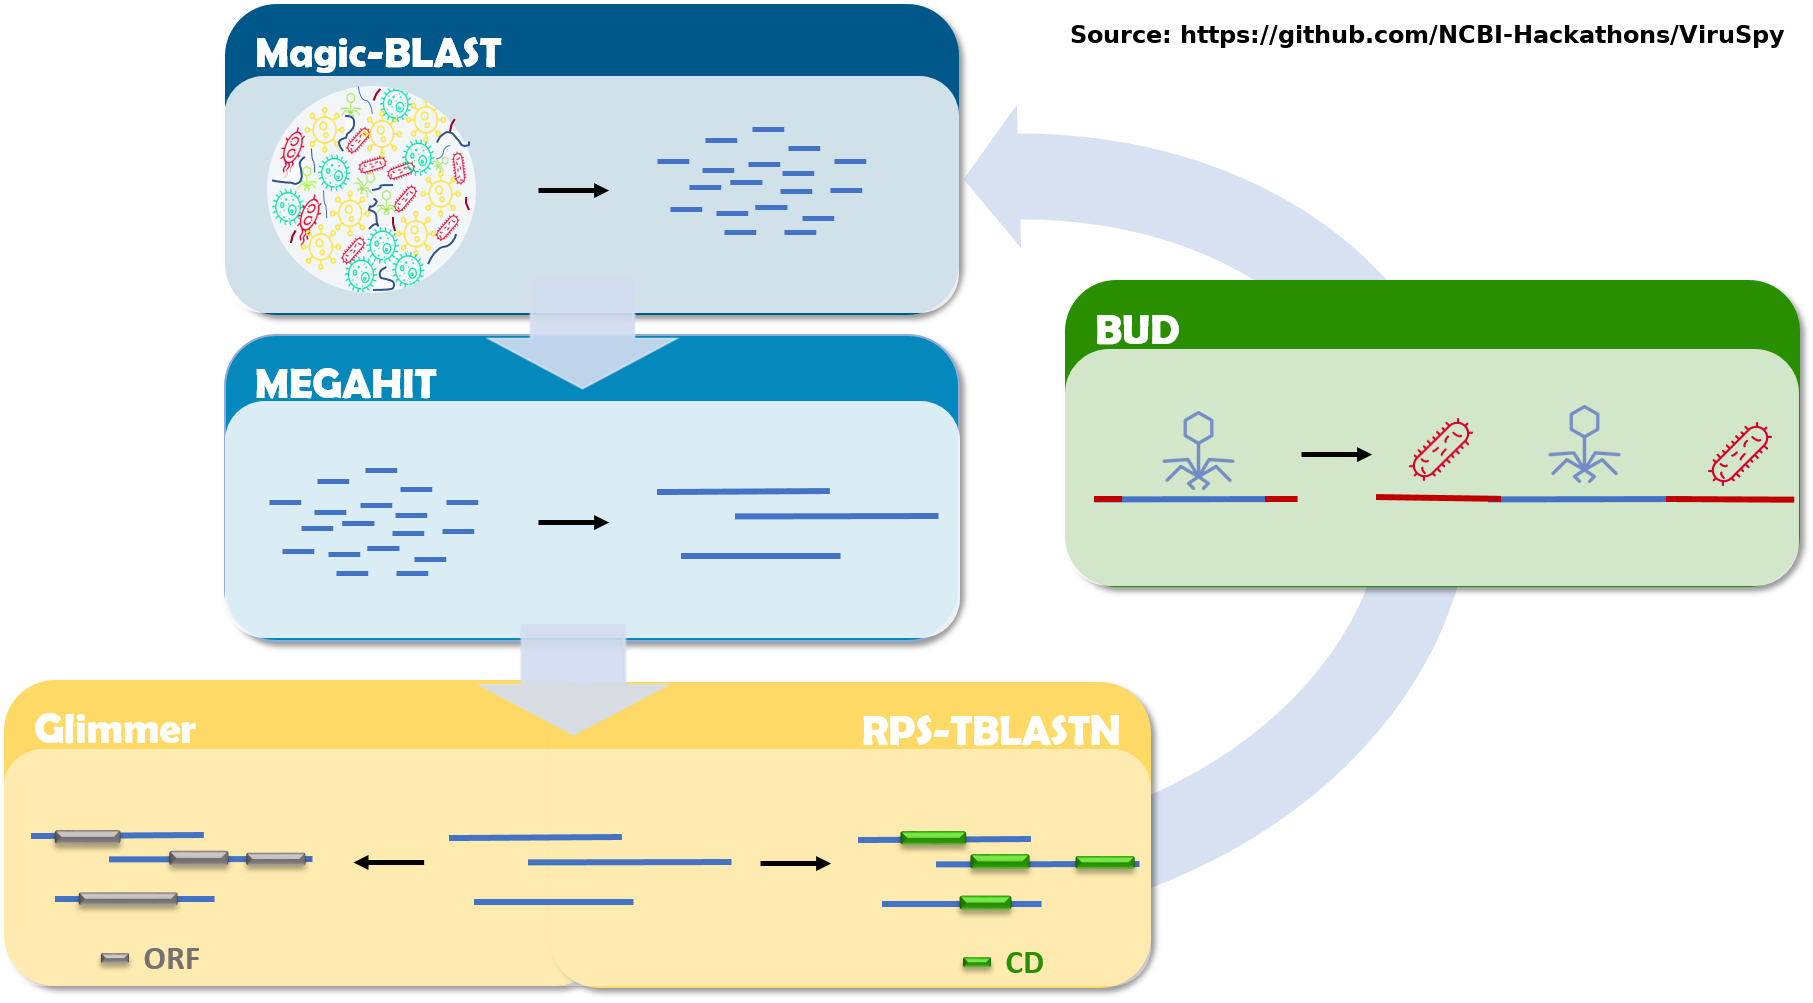
\includegraphics[width=\linewidth]{figs/bud_algo.jpg}
  \end{frame}


  \begin{frame}{Endovir}
    \resizebox{\linewidth}{!}{%% https://tex.stackexchange.com/questions/62262/legend-in-tikzpicture
% argument #1: any options
\newenvironment{customlegend}[1][]{%
    \begingroup
    % inits/clears the lists (which might be populated from previous
    % axes):
    \csname pgfplots@init@cleared@structures\endcsname
    \pgfplotsset{#1}%
}{%
    % draws the legend:
    \csname pgfplots@createlegend\endcsname
    \endgroup
}%

% makes \addlegendimage available (typically only available within an
% axis environment):
\def\addlegendimage{\csname pgfplots@addlegendimage\endcsname}

%%--------------------------------

% definition to insert numbers
\pgfkeys{/pgfplots/number in legend/.style={%
        /pgfplots/legend image code/.code={%
            \node at (0.125,-0.0225){#1}; % <= changed x value
        },%
    },
}

  \def\blockdist{0.3}
  \begin{tikzpicture}[>=latex,shorten >=2pt,shorten <=2pt]
    \pgfdeclarelayer{background}
    \pgfdeclarelayer{foreground}
    \pgfsetlayers{background,main,foreground}

    \node (mapper)    [tool] {magicBLAST};
    \node (refseq)    [db,  above = of mapper]    {RefSeq Virus};
    \node (sra)       [db,  below = of mapper]    {SRA};
    \node (fmapper)   [tool, below = of sra]      {magicBLAST};
    \node (asm)       [tool, right = of mapper]   {Assembler};
    \node (mscreen)   [tool, right = of asm]      {Motif screen};
    \node (reject)    [data, right = of mscreen]  {Rejected contigs};
    \node (flanker)   [func, right = of fmapper]  {Flanker};
    \node (ctgs)      [data, right = of flanker]  {Contigs};
    \node (cscreen)   [tool, below = of ctgs]     {Motif screen};
    \node (overlaps)  [func, left = of fmapper]   {Overlapper};
    \node (extend)    [func, below = of overlaps] {Extender};
    \node (ctgChk)    [func, right = of extend]   {Contig inspector};
    \node (ctgMerge)  [func, below = of cscreen]  {Contig merger};


    \path[->] (refseq)    edge (mapper)
              (sra)       edge (mapper)
                          edge (fmapper)
              (mapper)    edge (asm)
              (asm)       edge (mscreen)
              (mscreen)   edge (reject)
                          edge (ctgs)
              (ctgs)      edge (flanker)
              (flanker)   edge (fmapper)
              (fmapper)   edge (overlaps)
              (overlaps)  edge (extend)
              (extend)    edge (ctgChk)
              (ctgChk)    edge (cscreen)
                          edge (ctgMerge)
              (ctgMerge)  edge (cscreen)
              (cscreen)   edge (ctgs);

    \path[partLabel] (asm.north) +(0,+2*\blockdist) node (inital_desc) {Initial run};
    \path[partLabel](flanker.north) +(0,+2*\blockdist) node (bud) {BUD};
    \begin{pgfonlayer}{background}
      \path (mapper.west |- mapper.north)+(-0.3, \blockdist) node (a) {};
      \path (mscreen.south -| mscreen.east)+(+0.3,-0.3) node (b) {};


      \path (overlaps.west |- overlaps.north)+(-0.3, \blockdist) node (c) {};
      \path (ctgMerge.south -| ctgMerge.east)+(+0.3, -0.3) node (d) {};
      \path[partLabel]
          (a) rectangle (b);
      \path[partLabel]
          (c) rectangle (d);
    \end{pgfonlayer}
    \begin{customlegend}[legend cell align=left, %<= to align cells
                         legend entries={ % <= in the following there are the entries
                                           External tools,
                                           Database},
                         legend style={at={(10,-5)},font=\footnotesize}] % <= to define position and font legend
    % the following are the "images" and numbers in the legend
        \addlegendimage{area legend}
        \addlegendimage{mark=db, draw=white}
    \end{customlegend}
  \end{tikzpicture}
}
  \end{frame}

  \begin{frame}{Usage}
    \lstinputlisting{listings/usage.raw}

  \end{frame}

  \begin{frame}{Modularity}
    \begin{itemize}
     \item Facilitating extending and adding other tools using classes
           which act as messenger between tool and Endovir.
    \end{itemize}
    \lstinputlisting[language=Python,firstline=8]{listings/magicblast_alignment.py}

  \end{frame}

  \begin{frame}{Init}
    \resizebox{\linewidth}{!}{\documentclass[border=10pt]{standalone}
\usepackage{tikz}
\usetikzlibrary{shapes.geometric, positioning}

\tikzset{%
  db/.style = {cylinder, draw},
  tool/.style = {rectangle, draw},
  data/.style = {},
  func/.style = {},
  fake/.style = {}
}


\begin{document}
  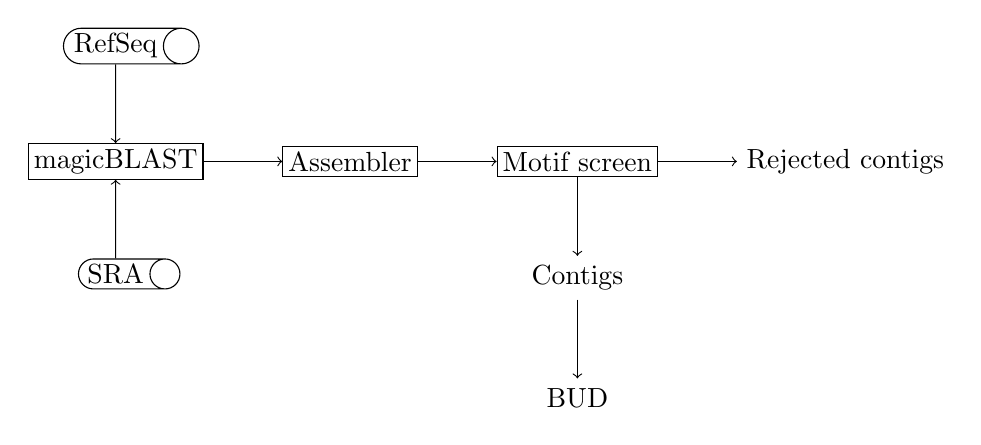
\begin{tikzpicture}
    \pgfdeclarelayer{background}
    \pgfdeclarelayer{foreground}
    \pgfsetlayers{background,main,foreground}

    \node (mapper)    [tool] {magicBLAST};
    \node (refseq)    [db,  above = of mapper] {RefSeq};
    \node (sra)       [db,  below = of mapper] {SRA};
    \node (asm)       [tool, right = of mapper]             {Assembler};
    \node (mscreen)   [tool, right = of asm]                {Motif screen};
    \node (reject)    [data, right = of mscreen]            {Rejected contigs};
    \node (ctgs)      [data, below = of mscreen]            {Contigs};
    \node (bud)       [func, below = of ctgs]               {BUD};

    \path[->] (refseq)    edge (mapper)
              (sra)       edge (mapper)
              (mapper)    edge (asm)
              (asm)       edge (mscreen)
              (mscreen)   edge (reject)
                          edge (ctgs)
              (ctgs)      edge (bud);
    %\begin{pgfonlayer}{background}
      %\path (mapper.west |- mapper.north)+(-0.5,0.3) node (a) {};
      %\path (mapper.south -| wa.east)+(+0.5,-0.3) node (b) {};
      %\path (vote.east |- asrs.east)+(+0.5,-0.5) node (c) {};

      %\path[fill=yellow!20,rounded corners, draw=black!50, dashed]
          %(a) rectangle (c);
      %\path (asr1.north west)+(-0.2,0.2) node (a) {};
    %\end{pgfonlayer}

  \end{tikzpicture}
\end{document}
}
  \end{frame}

  \begin{frame}{Bud}
    \resizebox{\linewidth}{!}{ \begin{tikzpicture}[>=latex,shorten >=2pt,shorten <=2pt]

    \node (sra)       [db,  below = of mapper]    {SRA};
    \node (fmapper)   [tool, below = of sra]      {magicBLAST};
    \node (flanker)   [func, right = of fmapper]  {Flanker};
    \node (ctgs)      [data, right = of flanker]  {Contigs};
    \node (cscreen)   [tool, below = of ctgs]     {Motif screen};
    \node (overlaps)  [func, left = of fmapper]   {Overlapper};
    \node (extend)    [func, below = of overlaps] {Extender};
    \node (ctgChk)    [func, right = of extend]   {Contig inspector};
    \node (ctgMerge)  [func, below = of cscreen]  {Contig merger};


    \path[->] (sra)       edge (fmapper)
              (ctgs)      edge (flanker)
              (flanker)   edge (fmapper)
              (fmapper)   edge (overlaps)
              (overlaps)  edge (extend)
              (extend)    edge (ctgChk)
              (ctgChk)    edge (cscreen)
                          edge (ctgMerge)
              (ctgMerge)  edge (cscreen)
              (cscreen)   edge (ctgs);
  \end{tikzpicture}
}
  \end{frame}

  \begin{frame}{Flanker}
    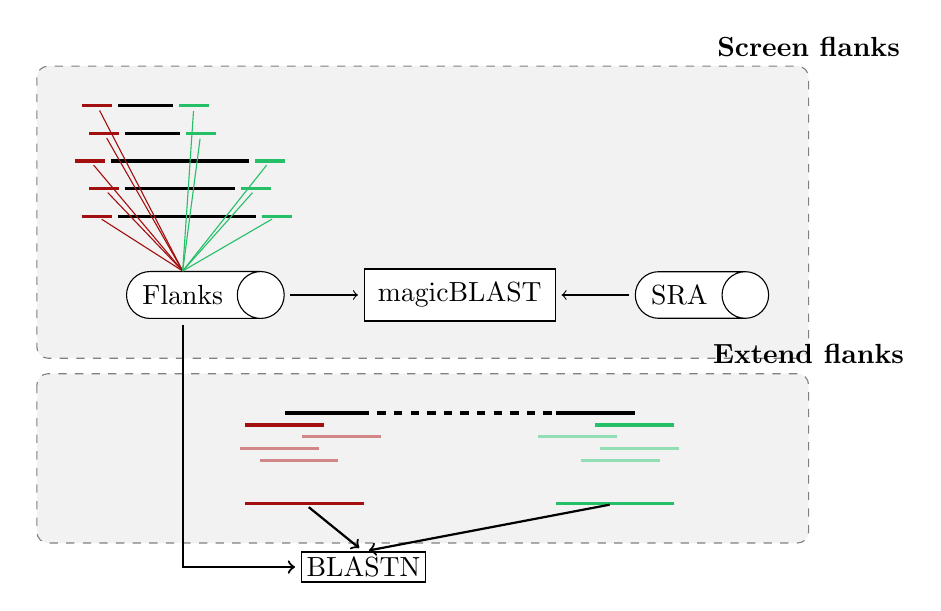
\begin{tikzpicture}%[>=latex,shorten >=2pt,shorten <=2pt]
 \tikzset
 {
  box/.style = {fill=gray!10,rounded corners, draw=black!50, dashed},
  boxtxt/.style = {font=\bfseries}
 }
  \pgfdeclarelayer{background}
  \pgfdeclarelayer{foreground}
  \pgfsetlayers{background,main,foreground}



  \begin{scope}[yshift=3em]
    \node (db) [db, inner sep=0.5em] at (1,-1) {Flanks};
  \node (mb) [tool, inner sep=0.5em, right = of db]  {magicBLAST};
  \node (sra) [db, inner sep=0.5em,right = of mb] {SRA};

    \def\n {4}
    \coordinate (lf) at (-3em, \n/2/\n);
    \coordinate (rf) at (9 em, \n/2/\n);
    \foreach \y in {0,...,\n}
    {
      \pgfmathsetmacro{\Xa}{(random(\n)/\n)}
      \pgfmathsetmacro{\len}{random(2,5)+\Xa}
      \pgfmathsetmacro{\lb}{\Xa-0.15em}
      \pgfmathsetmacro{\rb}{\len+0.15em}
      \coordinate (lb) at (\lb em, \y  em);
      \coordinate (ctgA) at (\Xa em, \y em);
      \coordinate (ctgB) at (\len em, \y em);
      \coordinate (rb) at (\rb em, \y em);
      \draw[leftfl, shorten >=2pt,shorten <=2pt, dna] (lb) -- (ctgA);
      \draw[dna] (ctgA) -- (ctgB);
      \draw[dna, rightfl, shorten >=2pt,shorten <=2pt] (ctgB) -- (rb);
      \draw[leftfl, shorten <=2pt] ($(lb)!0.5!(ctgA)$) -- (db.north);
      \draw[rightfl, shorten <=2pt] ($(ctgB)!0.5!(rb)$) -- (db.north);
    }
    \path[->, shorten >=2pt,shorten <=2pt]
      (db)  edge (mb)
      (sra) edge (mb);
    \begin{pgfonlayer}{background}
      %\path[box] (asm.north) +(0,+2*\blockdist) node (inital_desc) {Initial run};
      \path (lb.west |- lb.north)+(-0.5, 0.5) node (a) {};
      \path (sra.south -| sra.east)+(+0.5,-0.5) node (b) {};
      \path[boxtxt] (a -| b)+(0, 0.25) node (t.east) {Screen flanks};
      \path[box]
          (a) rectangle (b);
    \end{pgfonlayer}
  \end{scope}

  \begin{scope}[yshift=3em]
    \coordinate (A) at ($ (mb.east)+(0, -1.5)$);
    \coordinate (B) at ($ (mb.east)+(1, -1.5)$);
    \coordinate (Z) at ($ (mb.west)+(0, -1.5)$);
    \coordinate (Y) at ($ (mb.west)+(-1, -1.5)$);
    \draw[dna] (A) -- (B);
    \draw[dna, dashed] (B) -- (Z);
    \draw[dna] (Z) -- (Y);

    \def\n {4}
    \def\sp {0.15}
    \coordinate (K) at ($ (A)+(0.5, -\sp)$);
    \coordinate (L) at ($ (B)+(0.5, -\sp)$);
    \coordinate (Q) at ($ (Z)+(-0.5, -\sp)$);
    \coordinate (R) at ($ (Y)+(-0.5, -\sp)$);
    \draw[dna, rightfl](K) -- (L);
    \draw[dna, leftfl](Q) -- (R);
    \foreach \y in {2,...,\n}
    {
      \pgfmathsetmacro{\Xa}{(random()-0.3}
      \coordinate (C) at ($ (A)+(\Xa, -\y*\sp)$);
      \coordinate (D) at ($ (B)+(\Xa, -\y*\sp)$);
      \coordinate (V) at ($ (Z)+(-\Xa, -\y*\sp)$);
      \coordinate (W) at ($ (Y)+(-\Xa, -\y*\sp)$);
      \draw[dna, rightfl!50] (C) - - (D);
      \draw[dna, leftfl!50] (V) - - (W);
    }

    \coordinate (0) at ($(L)+(0,-1)$);
    \coordinate (1) at ($(A)+(0,-1.15)$);
    \coordinate (2) at ($(R)+(0,-1)$);
    \coordinate (3) at ($(Z)+(0,-1.15)$);

    \draw[dna, rightfl] (0) -- (1);
    \draw[dna, leftfl] (2) -- (3);

    \begin{pgfonlayer}{background}
      \path (Y -| a)+(0, 0.5) node (z) {};
      \path (1 -| b)+(0, -0.5) node (y) {};
      \path[boxtxt] (z -| y)+(0, 0.25) node (t.east) {Extend flanks};
      \path[box]
          (z) rectangle (y);
    \end{pgfonlayer}
  \end{scope}

  \begin{scope}
    \node [tool] (blast) [below = 5em of Z.west] {BLASTN};
    \draw[->, shorten >=2pt,shorten <=2pt, thick] (db) |- (blast);
    \draw[->, shorten <=2pt,shorten >=2pt, thick] ($(0)!0.5!(1)$) -- (blast.north);
    \draw[->, shorten >=2pt,shorten <=2pt, thick] ($(2)!0.5!(3)$) -- (blast.north);
  \end{scope}
\end{tikzpicture}

  \end{frame}

  \begin{frame}{Outlook}
    \begin{itemize}
     \item Adjust tool parameters on the fly
     \item Replace SRA toolkit with NCBI's ngs-python
     \item Test on more diverse datasets
    \end{itemize}
  \end{frame}

\end{document}
